\classheader{11-17-2017}


\section*{The Fundamental Group is a Homotopy Invariant}
Homotopy is a more general quality than homeomorphism.  Whereas a homeomorphism requires the existence of a continuous bijection with continuous inverse, we say that $X$ and $Y$ are homotopy equivalent if there exist continuous functions $f:X\rightarrow Y$ and $g:Y\rightarrow X$ such that $f\circ g$ is homotopic to the identity on $Y$ and $g\circ f$ is homotopic to the identity on $X$.

For example, the closed disk and a single point are homotopic, but obviously not homeomorphic.  Similarly, $\R^n$ is homotopic to a single point.  Also, $\R^n{-}\{0\}$ is homotopic to $\S^{n-1}$ by the maps $f(x)=x/||x||$ and $g(y)=y$.

Homotopy equivalence is an equivalence relation.  We've seen how it's obviously reflexive and symmetric, but it is transitive as well, via composition of functions.

\begin{theorem}
	The fundamental group $\pi_1$ is a homotopy invariant.  That is, if $X$ and $Y$ are each path connected and homotopy equivalent to each other, their fundamental groups are isomorphic.
\end{theorem}
\begin{proof}
	We proceed in two steps:
	
	\textbf{Step I:} First we'll show that if $h_t:X\rightarrow X$ is a homotopy then for any $t\in[0,1]$ we have $\pi_1(X,x_0)\iso \pi_1(h_t(X),h_t(0))$.
	
	\textbf{Proof:} If $[\gamma]\in\pi_1(X,x_0)$ is a class of loops in the fundamental group of $X$, then $[h_t\circ\gamma]\in \pi_1(h_t(X),h_t(x_0))$ is a class of loops in the fundamental group of the image of $X$ under $h_t$.  Furthermore, the map $h_{t*}$ which sends $[\gamma]$ to $[h_t\circ\gamma ]$ is a homomorphism of groups by the theorem from last time.  
	
	Let $\phi^t$ be the path homotopy which moves $X$ to $h_t(X)$, as in the following diagram.  We can then compose this to describe  a path homotopy $H(s,t) = (\phi^{t})^{-1}\circ (h_t\circ \gamma)\circ \phi^t (s)$\\
	
	\begin{figure}[!htb]
		\centering
		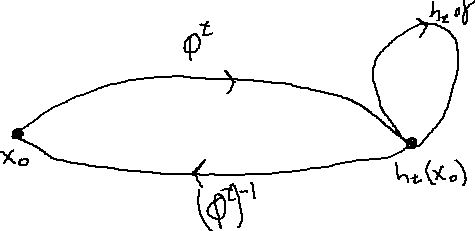
\includegraphics[scale=.5]{images/hst_hom}
		\caption{The $\phi^t$ homotopy}
		\label{fig:hst_hom}
	\end{figure}
	
If $h_t\circ\gamma$ is null homotopic, then we can contract this whole loop and see that $(\phi^{t})^{-1}\circ (h_t\circ \gamma)\circ \phi^t$ is null homotopic as well, thus the kernel of this map is trivial and it is injective.

To see that it is surjective, let $[\eta]$ be a class of loops in $\pi_1(h_t(X),h_t(x_0)$, and we'll show that there is something in $\pi_1(X,x_0)$ which maps to it.

To do this, we can use the same homotopy $\phi^t$, but we'll go the other way.  If $\eta$ is a loop in $\pi_1(h_t(X),h_t(x_0))$, then $(\phi^{t})^{-1}\circ \eta\circ \phi^t$ is a loop in $\pi_1(X,x_0)$.  Thus $h_{t*}([(\phi^{t})^{-1}\circ \eta\circ \phi^t]) = [\eta]$, and the map is surjective as well.  Thus we have a homomorphism of groups which is setwise bijective, and it is an isomorphism.

\qed

\textbf{Step II:} If $f:X\rightarrow Y$ and $g:Y\rightarrow X$ form a homotopy equivalence between path connected spaces, then

$$f_*:\pi_1(X,x_0)\rightarrow \pi_1(Y,y_0)$$
$$g_*:\pi_1(Y,y_0)\rightarrow \pi_1(X,x_0)$$

are isomorphisms of groups.

\textit{Proof:} The composition
$$\pi_1(X,x_0)\xrightarrow{f_*}\pi_1(f(X),f(x_0)\xrightarrow{g_*}\pi_1(g(f(X)),g(f(x_0))) \xrightarrow{\iso}\pi_1(X,x_0)$$
is a group isomorphism by Step I.  Since $(g\circ f)(x)$ is homotopic to the identity on $X$ and $X$ is path connected, we can change the base point without issue.

Thus $g_*\circ f_* = (g\circ f)_*$ is homotopic to the identity, and it is an isomorphism from $\pi_1(X,x_0)$ to itself. We have that $f_*$ is injective and $g_*$ is surjective, and we can exchange $f$ and $g$ to see the opposite, so $f_*$ and $g_*$ are bijective group homomorphisms, so they are isomorphisms.
\end{proof}
